% Pursuing Stacks (cotes 134-2 to 134-8): archive cote 134-2, site page 27 (PDF page 28).
% letter to Quillen. Draft compared: ps1.tex:607-682.
% AI-transcribed by Claude Opus 5.5 (claude-opus-5-5, adaptive thinking, effort high), Message Batches API, batch ps1 (msgbatch_01Rv5hCaNTtUt4JHx1yqoHPL), 2026-11-12; not yet checked by eye.
\scanpage{134-2/27}
\mspage{\deleted{\illegible{1}} 13}
\margin{\unsure{1}}

understood that the"amalgamated sums"\inserted{(rather, finite \unsure{$\varinjlim$'s})} we are considering are of the most
common type,  when X is the finite union of closed subset\xout{\unsure{s}} $X_i$ ,  with
given isomorphisms
\[ X_i \simeq D_{n(i)} \quad , \]
the intersection of any two of these $X_i \cap X_j$ being a union of closed \deleted{cell}\inserted{cells}
both in $D_{n(i)}$ and in $D_{n(j)}$ . (This implies in fact that it is either
\margin{(\unsure{12}!)).} a closed cell\xout{\unsure{s}} in both,  or the union of two closed cells of same dimens\hand{\unsure{ion}}
m and hence isomorphic to $S_m$ , a case which will be ruled out anyhow
by the triviality condition \deleted{\illegible{3}} which follows.\inserted{(12)}\deleted{\illegible{2}})The triviality or "standar\unsure{t}-%
\margin{\unsure{Salut}? \unsure{Absurde} \diagram{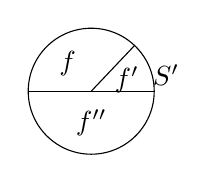
\begin{tikzpicture}\draw (0,0) circle (0.8); \draw (-0.8,0)--(0.8,0); \draw (0,0)--(0.55,0.58); \node at (-0.3,0.35) {$f$}; \node at (0.45,0.15) {$f'$}; \node at (0,-0.4) {$f''$}; \node at (0.95,0.2) {$S'$};\end{tikzpicture}} $f \cap f'' = S_0$}
ness" condition is now expressed by demanding that the set of indices
I can be totally ordered, \inserted[typed]{i.e. numbered} in such a way that we get X by succesively
"attaching" \unsure{Dells|cells} $D_{n(i)}$ to the space already constructed\xout{\unsure{,}} X(i-1), by a
map from \deleted{a}\inserted{a sub-} cell \xout{$D_i$}\inserted{of $D_{n(i)}$}, $S_j^{\hand{\varepsilon}} \to X(i-1)$ \quad $(\hand{\varepsilon\in\{}\pm 1\hand{\}})$ , this map of course
inducing an isomorphism,  more precisely \uline{the} standard isomorphism,\inserted{$\varphi^{\unsure{\varepsilon'}}_{n(i)}$}\deleted{of}
\margin{$\varphi^{\varepsilon'}_{n(i),j}$}
$S_j^{\hand{\varepsilon}} \simeq D_j$ \quad with\inserted{$S^{\varepsilon'}_j$} one of the two corresponding cells $S_j^+$ , $S_j^-$ in some
\margin{$S^{\varepsilon'}_j$}
$X_{i'} \simeq D_{n(i')}$ .  The \xout{xxxxx} dual translation of this\hand{,}in terms of fiber
products in \xout{xxx} a category C endowed with objects $F_i$ $(i\in\underline{N})$ and maps
$s_1^i , t_1^i$ between these, is clear:  for a given set of indices I and map
\margin{$P=\prod_{i\in I}F_{n(i)}$}
$i \mapsto n(i) : I \to \underline{N}$ , we consider a sub\xout{xxx}\inserted{-object of} $\inserted{P=}\hand{\prod_{i\in I}}F_{n(i)}$ ,  which can be
described by equality relations between it\over{t}{e}rated sources and targets
\xout{xxxxxx} of various components of $u = (u_i)_{i\in I}$  in P,  the structure of
the set of relations being such that I can\hand{\unsure{,}}be numbered, from 1 to N say,
in such a way that we get in succession \deleted{N}\inserted{$N-1$} relations on the N components
$u_i$ respectively,\inserted{$(2\leq i \leq N)$} every relation being of the type $f(u_i) = g(u_{i'})$ , with
f and g being iterated source or target maps, and $i'<i$ . \hand{(Whether}
\hand{source or target depending in obvious way on the two signs $\varepsilon,\varepsilon'$)}

\mspage{27}
